\chapter{Introduction}
Since life's first beginnings, nature has been seeking optimal solutions to surviving in a constantly changing environment.
One key adaptation towards this goal, as evidenced by the ubiquity with which it is found throughout the tree of life, is the ability of an organism to anticipate daily changes to its environment.
Such rhythms are known as {\itshape circadian}, and are classified by a number of defining characteristics \cite{Dunlap2009}:

\begin{itemize}
  \item They are {\em endogenous}, meaning they continue to oscillate even when the organism is isolated from its environment.

  \item They are temperature compensated, maintaining a consistent period for moderate changes in average temperature.

  \item They are {\em entrainable}, meaning they can adjust their phase and period in response to a changing in environmental signal.

  \item They oscillate with a roughly 24 hour period.
\end{itemize}

In this thesis, I apply techniques from systems biology in order to gain a more thorough understanding of how circadian rhythms control mammalian physiology, and how these rhythms might be altered through pharmacological therapies. % Really for abstract
Systems biology is a multidisciplinary field, drawing from biology, mathematics, and computer science. 
In this chapter, I first provide a background on the biology of circadian rhythms, followed by an introduction to the mathematical techniques which have been used to study them. 
I also discuss some computational considerations in the estimation of model parameters.

\section{Biological background}

\subsection{Dynamics of gene expression}

In the central dogma of molecular biology, genetic information is passed from DNA to mRNA to protein. 
While each cell in a multi-celled organism contains nearly identical DNA, the rate with which different genes are expressed results in substantial differences in cell type and function. 
These differences are the result of complex gene transcription networks, in which the production of some proteins - known as transcription factors - activate or repress the production of other genes. 
Similar to electrical circuits, network motifs such as positive and negative feedback arise from the interconnection of transcription factors.

Gene regulatory networks are essential to biological function. 
Cells maintain energy homeostasis by carefully balancing the flux of metabolites into energy storage and energy production pathways. 
These reactions are catalyzed by numerous enzymes, the activities of which must fluctuate to ensure the proper allocation of resources within a cell.
Enzyme production, degradation, and activation are controlled by transcription factors, and thus environmental conditions can be processed by complex network interactions to regulate metabolic function.
Circadian rhythms play a major role in the regulation of metabolic cycles, as periodic shifts in energy availability require a similar periodic shifts in gene transcription.



\subsection{Evolutionary history}

By looking at the evolutionary history of circadian rhythms, Edgar and colleges \cite{Edgar2012} demonstrated that cellular timekeeping may have began as a response to the Great Oxidation Event occurring $\approx 2.5$ billion years ago. 
Due to increased oxygen levels, the generation of reactive oxygen species in the cell can lead to oxidation of key biomolecules, prompting cells to express scavenging mechanisms during times of high UV light exposure. 
Over time, these pathways coupled to transcription-translation feedback loops in individual organisms, giving rise to a diverse set of circadian regulatory pathways (\fref{fig:edgarros}, from \cite{Edgar2012}). 

\begin{figure}[tbp]
  \centering
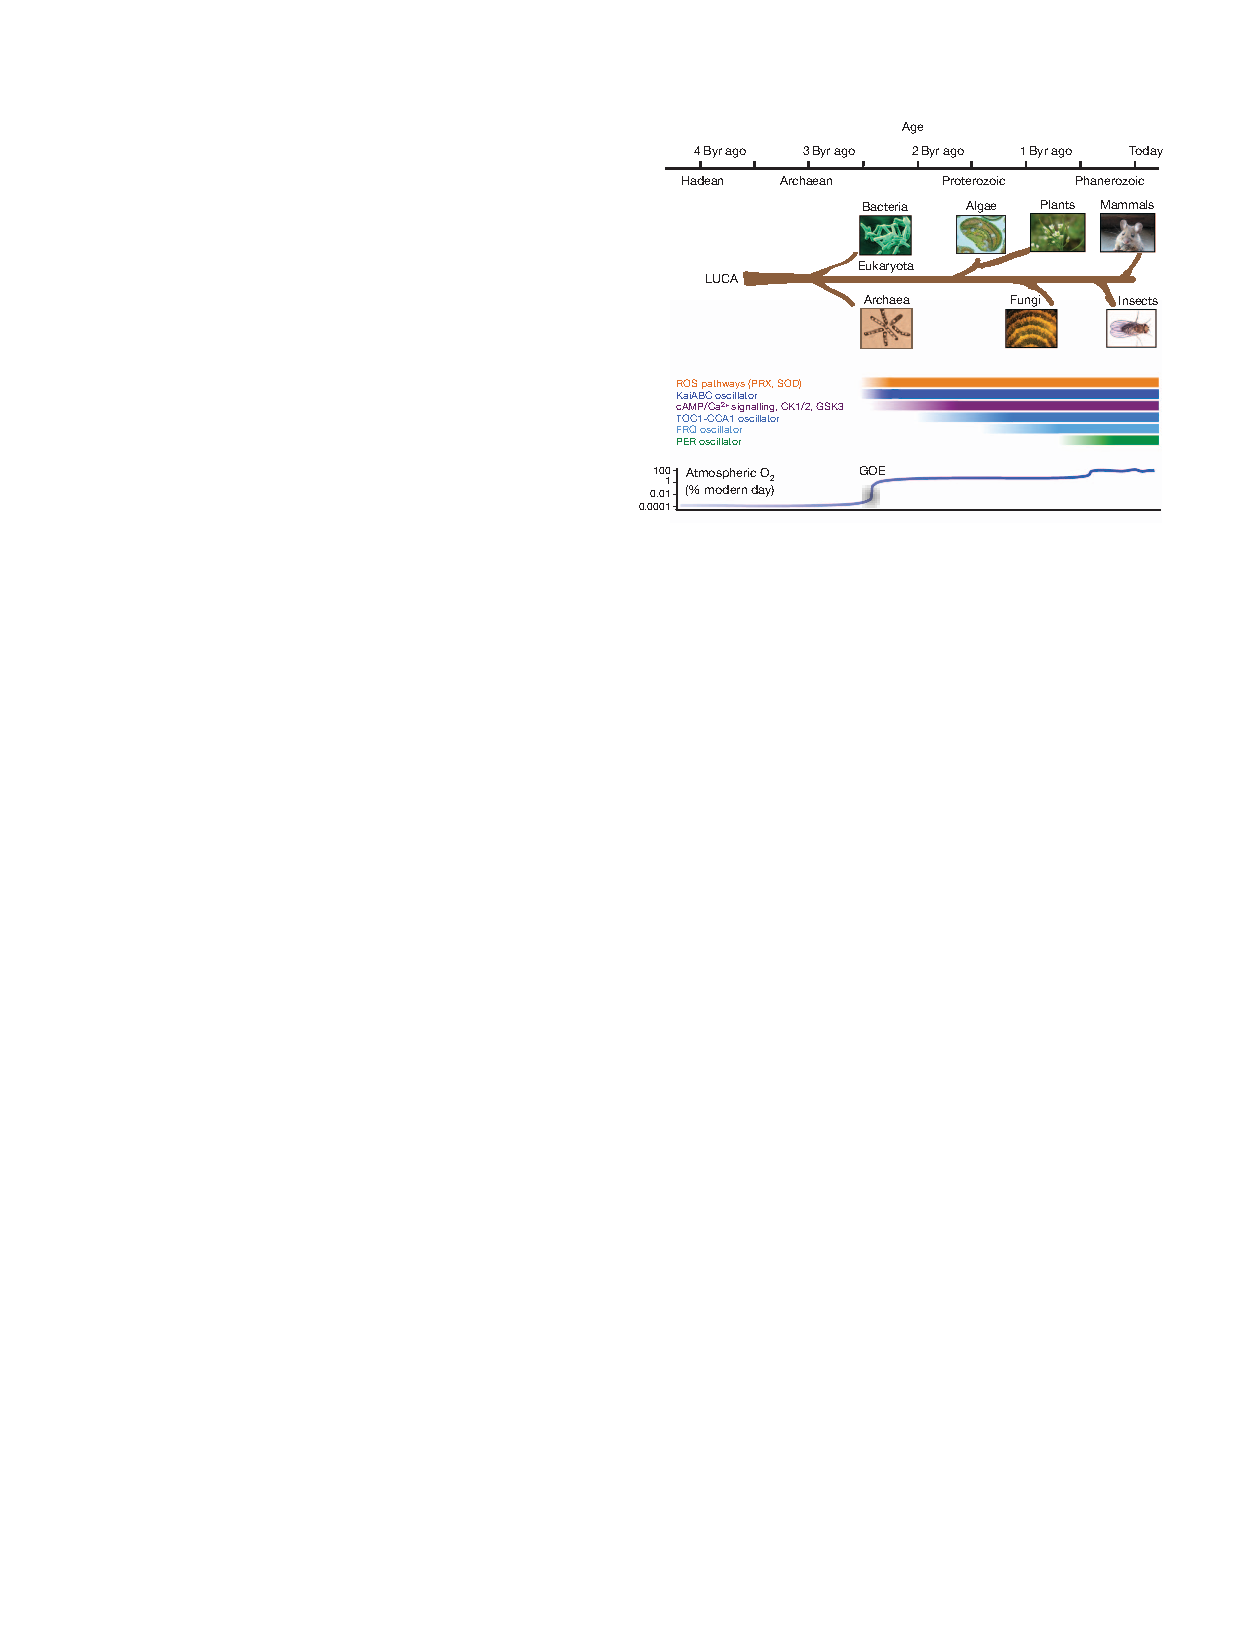
\includegraphics[width=0.8\textwidth]{chap1/figures/edgar_ros.pdf}
\titlecaption{Reactive oxygen species are conserved markers of circadian rhythms}{A timeline of the appearance of the main circadian feedback loops demonstrates that the rhythmic protection against light-mediated oxidation is a conserved rhythm across many evolutionary trees. Figure taken from \cite{Edgar2012}.}
  \label{fig:edgarros}
\end{figure}

\subsection{Circadian rhythms in mammals}

\subsubsection{Tissue-level clocks}

In mammals, circadian rhythms are organized in a hierarchical structure, in which inputs from the environment are processed separately by different tissue-level clocks (\fref{fig:feedforward}). 
Light, the primary entraining factor, is directed towards the suprachiasmatic nucleus (SCN), a tissue in the brain that serves as the body's master pacemaker \cite{Ralph1990}. 
In the SCN, approximately $20,000$ cells communicate via intercellular coupling to determine a precise internal time, which coordinates rhythms in locomotor activity \cite{Aton2005}.

\begin{figure}[tbp]
  \centering
  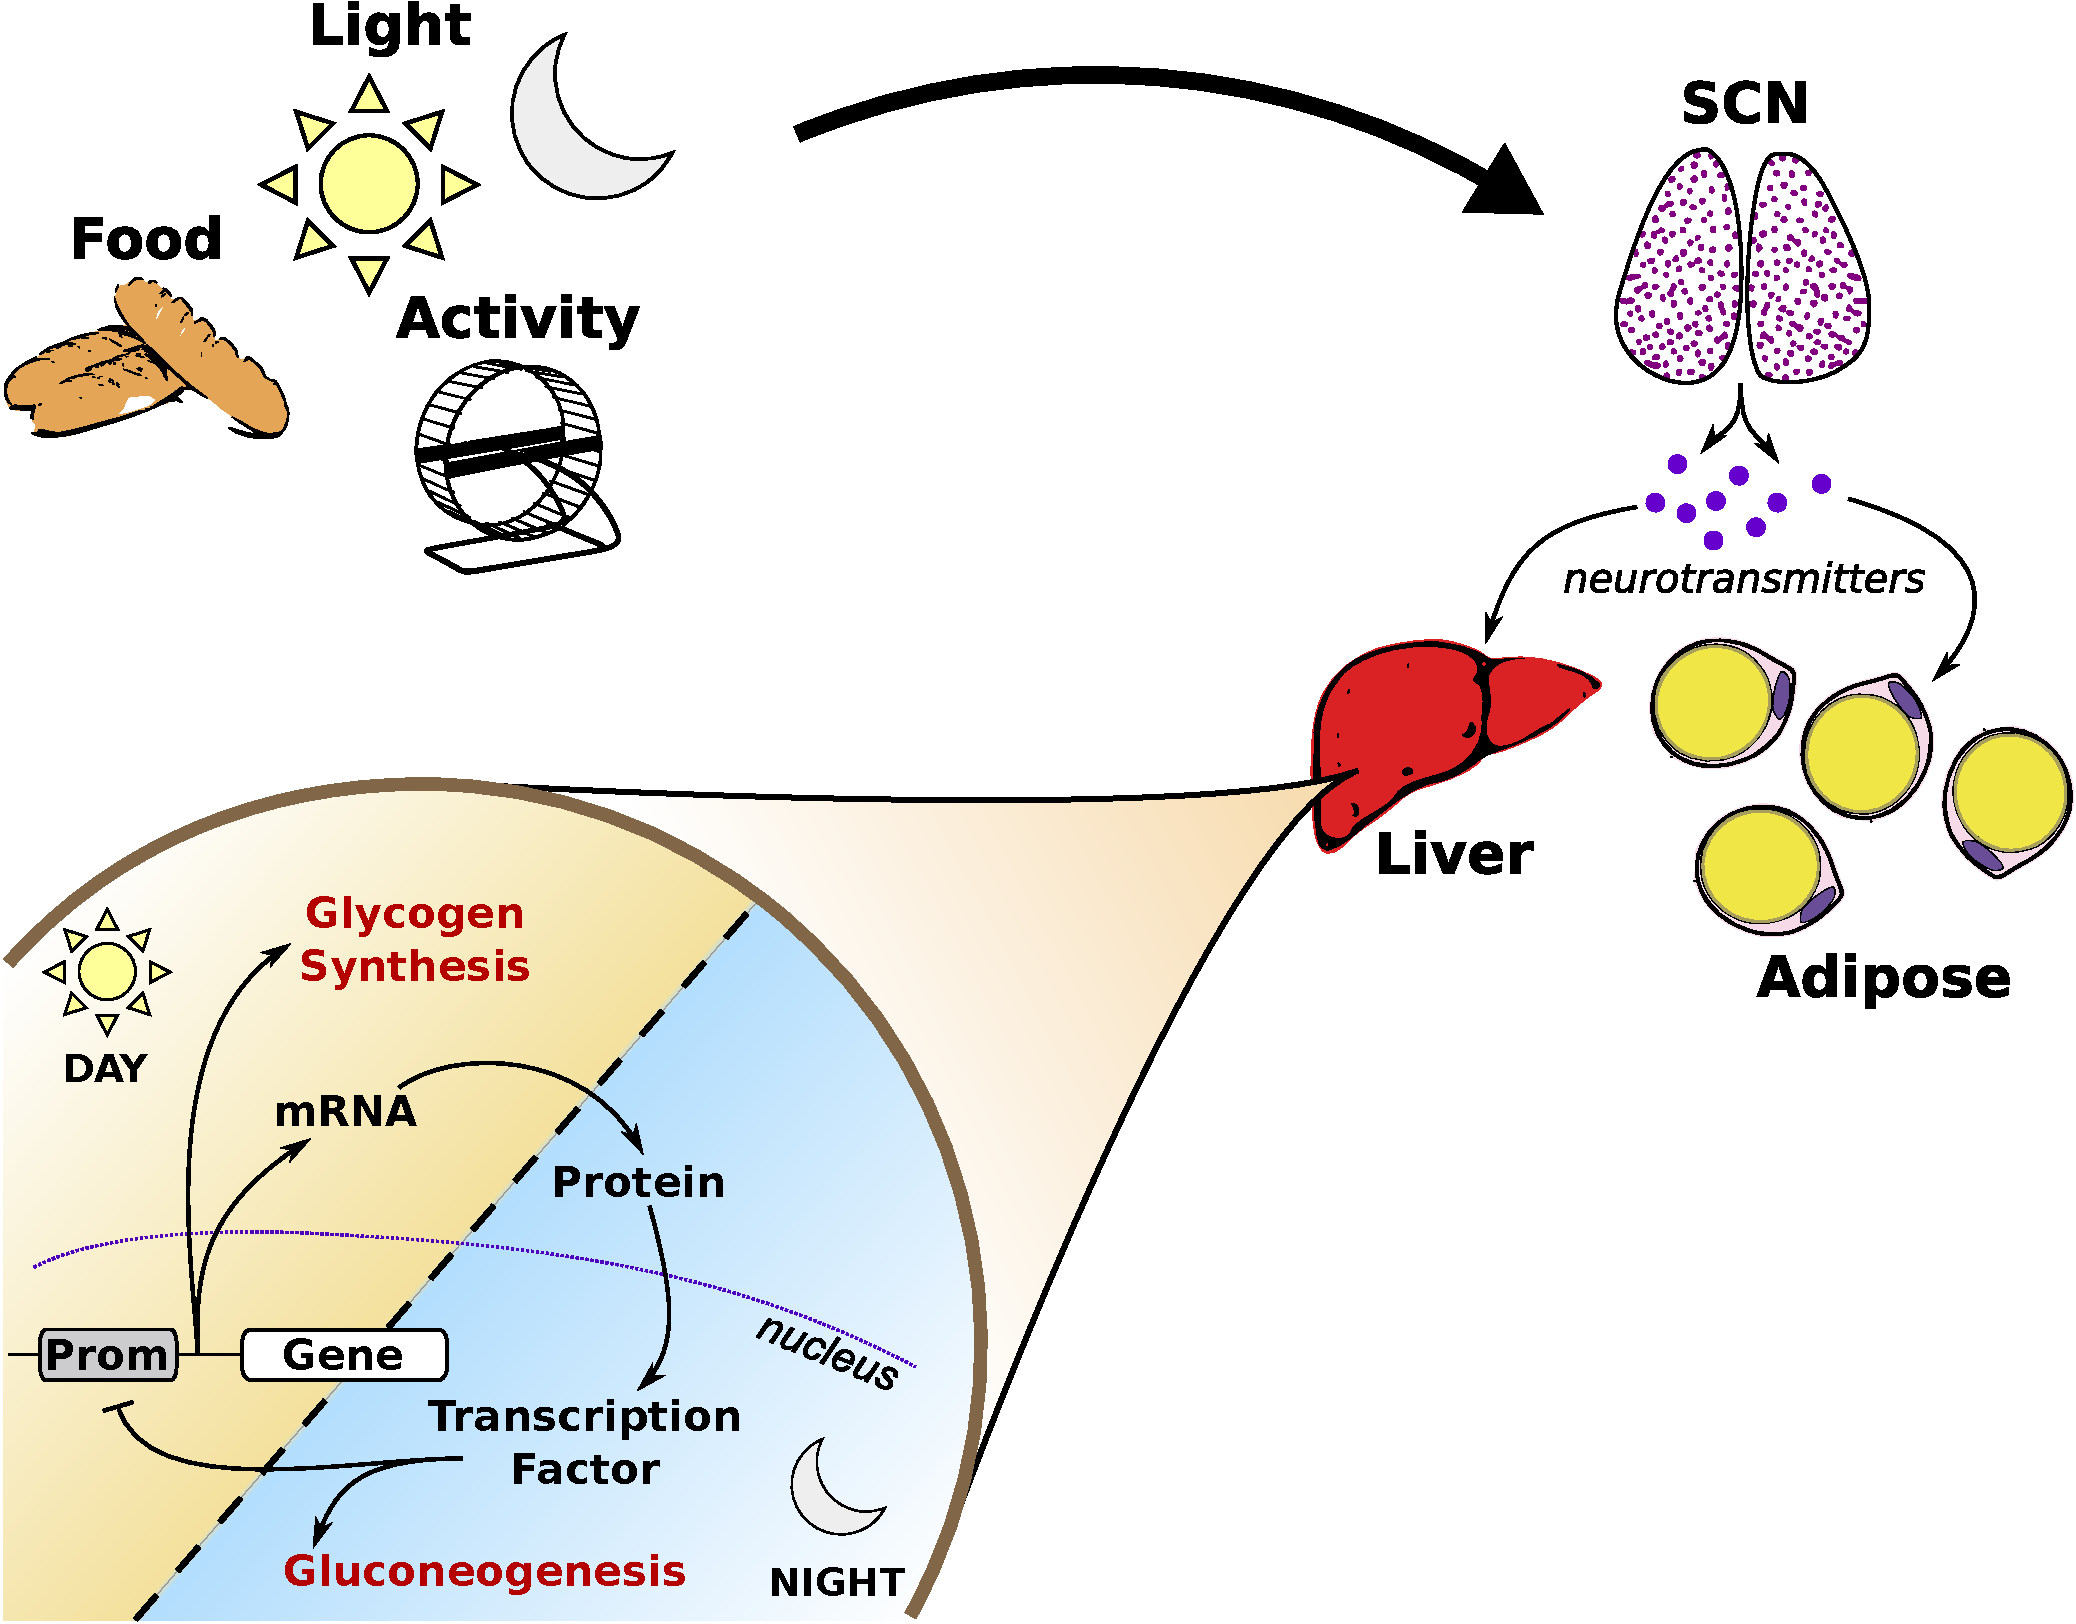
\includegraphics[width=\textwidth]{chap1/figures/timescale_separation.pdf}
  \titlecaption{A biological feed forward controller}{Circadian rhythms are organized in a hierarchical fashion, in which inputs from the environment are processed by different tissue-level clocks. At the single-cell level, rhythms are generated via a time-delayed transcription-translation negative feedback loop. Environmental inputs are used to predict upcoming environmental conditions by speeding or slowing the oscillatory cycle, matching the body's internal phase with the external environment.}
  \label{fig:feedforward}
\end{figure}

Peripheral tissues are responsible for responding to changes daily changes in food intake \cite{Bass2010}. 
Liver and adipose tissue, for instance, maintain robust circadian oscillations \cite{Yoo2004}, which respond mainly to temperature and food resetting cues \cite{Yamazaki2000a}.
Such clocks are important to maintaining metabolic health, as knockout experiments demonstrate that compromised circadian in peripheral tissues leads to many disorders, including diabetes and obesity \cite{Marcheva2010, Shi2013}.
Additionally, feeding cycles have been shown to have a profound impact on  circadian oscillations in peripheral tissues. High-fat or out of phase feeding leads to a reprogramming of oscillatory genes and metabolites 
\cite{Kohsaka2007, Hatori2012}, often leading to metabolic disease.

\subsubsection{Circadian oscillations at the single-cell level}
Circadian rhythms are generated at the single-cell level through genetic regulatory networks with inherent time-delayed negative feedback. 
Transcription factors CLOCK and BMAL1, peaking in the early night, activate expression of EBOX genes period ({\itshape Per1} and {\itshape Per2}) and cryptochrome ({\itshape Cry1} and {\itshape Cry2})\footnote{In this thesis, I denote mRNA species using italics, and protein products using all capital letters.}.
{\itshape Per} and {\itshape Cry} protein products, PER and CRY, peaking during the early day, form a heterodimeric complex to cross the nuclear membrane \cite{Ko2006}. 
However, since PER is present in the cytoplasm in much lower quantities than CRY, it is stochiometrically-limiting for nuclear entry \cite{Lee2001}. 
Once inside the nucleus, the PER-CRY complex dissociates, and CRY represses CLOCK-BMAL1 mediated activation of EBOX genes, leading to rhythmic gene expression.
Several time delays contribute to the 24 hour oscillatory period, highlighted in \fref{fig:maindelays}.

\begin{figure}[tbp]
  \centering
  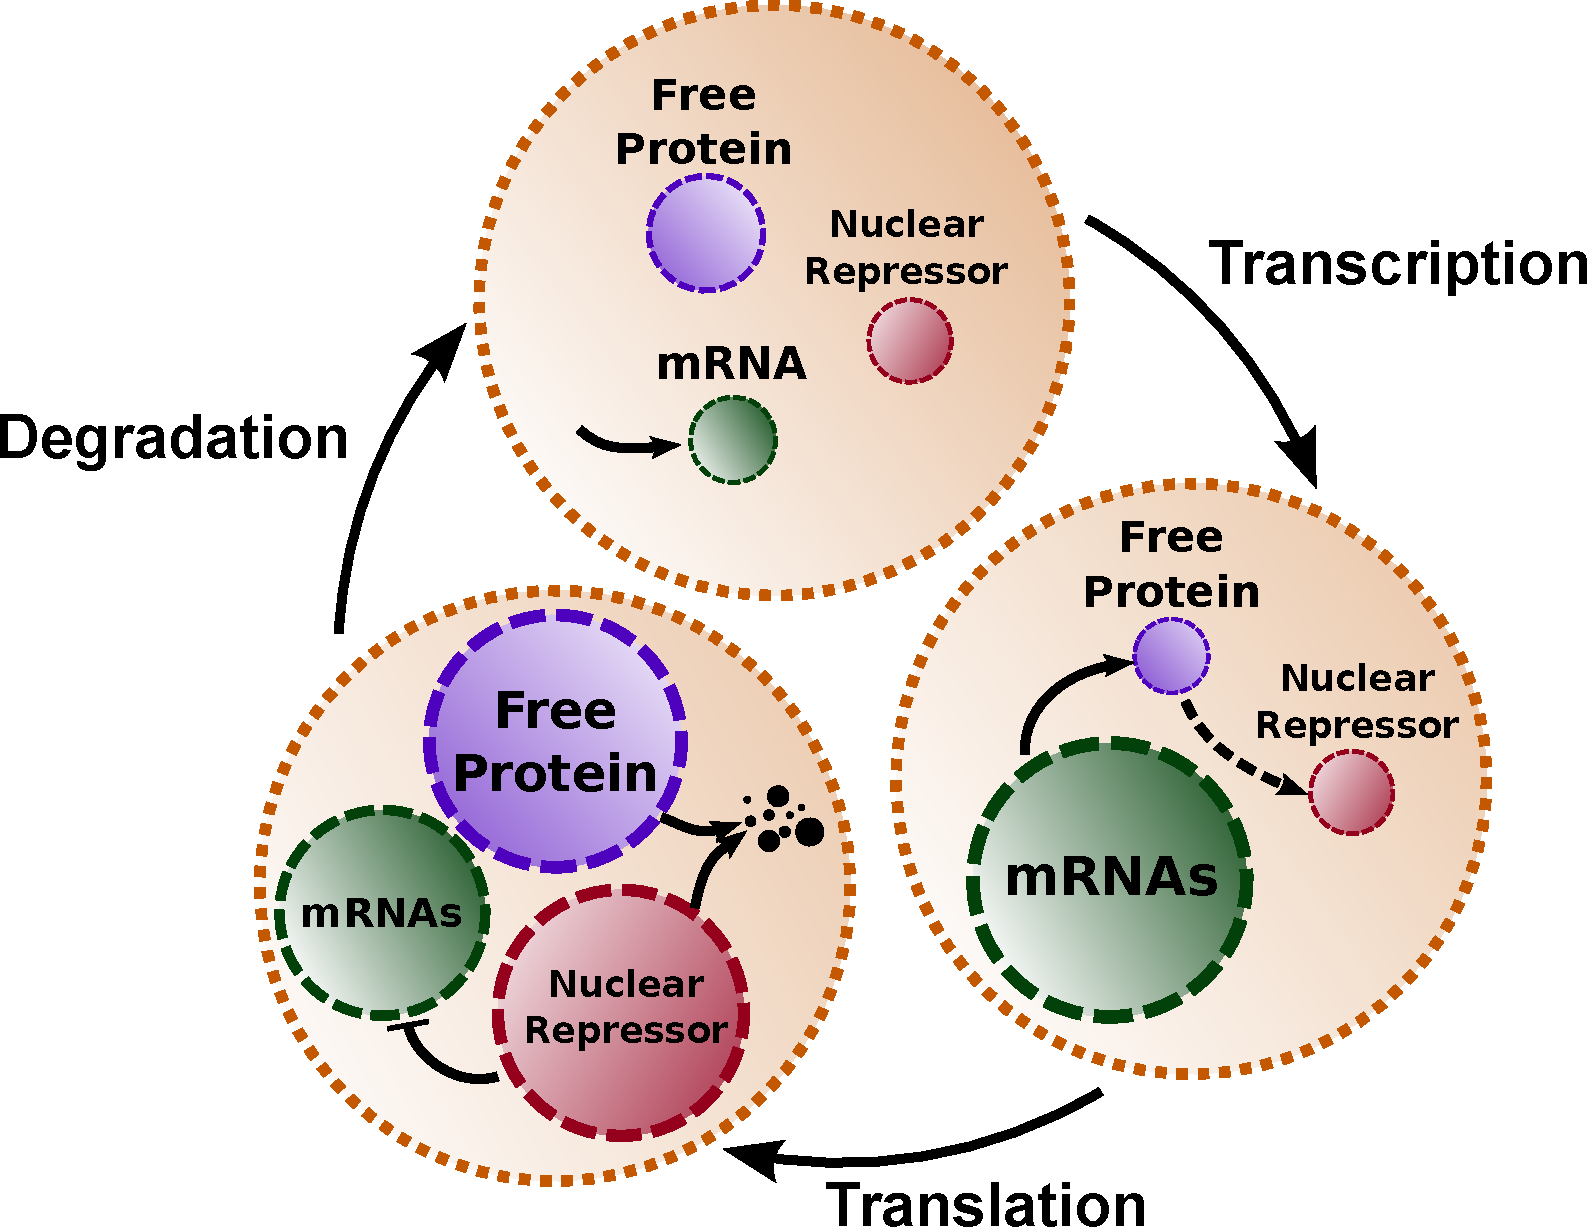
\includegraphics[width=0.7\textwidth]{chap1/figures/maindelays.pdf}
  \titlecaption{Key time delays}{Negative feedback may give rise to sustained oscillations in the presence of time delays. In the circadian system, these time delays are transcription, translation, and protein degradation. Each of these rates is a function of the external environment, resulting in entrainable oscillations.}
  \label{fig:maindelays}
\end{figure}

Additional components, namely the ROR and REV-ERB families of genes, add a layer of positive feedback to the clock regulatory loop.
This addition results in more reliable clock oscillations, as the bistability induced by the positive feedback stabilizes the negative-feedback induced oscillations \cite{Ananthasubramaniam2014a}.
A schematic of the core feedback in mammalian circadian rhythms is shown in \fref{fig:coreloop}.

\begin{figure}[tbp]
  \centering
  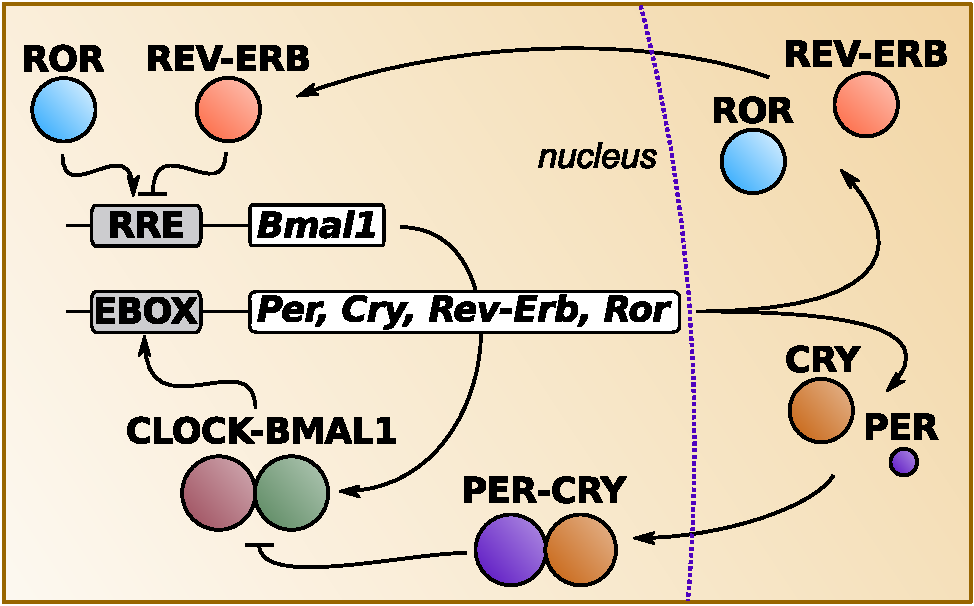
\includegraphics[width=0.7\textwidth]{chap1/figures/coreloop.pdf}
  \titlecaption{Core components of the mammalian circadian feedback loop}{The mammalian feedback loop is comprised of interlocking positive and negative feedback loops.}
  \label{fig:coreloop}
\end{figure}

\subsection{Experimental techniques}

While the focus of this thesis is primarily computational, I present a brief overview of the relevant experimental methods for studying circadian rhythms.
Most classical experiments determined the roles and importance of circadian genes using activity data of mouse knockouts \cite{Vitaterna1994}.
For instance, the period-determining effect of CRY1 and CRY2 were found by analyzing wheel-running behavior of mice in plots known as actograms \cite{VanderHorst1999}, as shown in \fref{fig:vanderhorst}.

\begin{figure}[tbp]
  \centering
  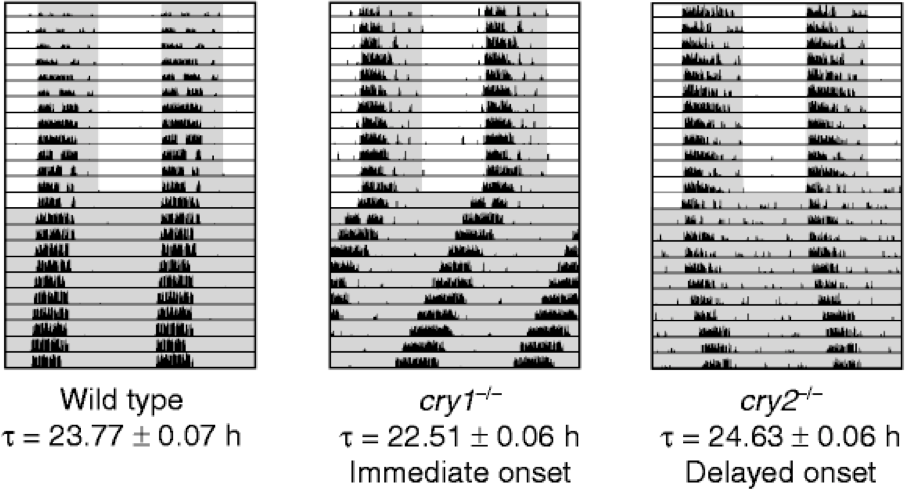
\includegraphics[width=0.7\textwidth]{chap1/figures/vanderhorst.png}
  \titlecaption{Period effects of CRY knockouts}{Actograms plot the intensity of mouse wheel-running activity. The x-axis plots time of day (data is double-plotted), while the y-axis shows each subsequent day. Black bars for each day indicate the intensity of wheel-running activity. After the mice are transferred to constant darkness, the free-running period can be inferred by fitting a line to the offset in activity onset each day. Figure taken from \cite{VanderHorst1999}.}
  \label{fig:vanderhorst}
\end{figure}

While activity-level knockout data is still used to characterize the effects of circadian perturbations, such methods are costly to implement and not amenable to high-throughput experimentation.
The development of luciferase reporter cell lines has rapidly changed the way circadian genes are screened \cite{Yoo2004}.
In reporter cells, the coupling of a luciferase protein to a core-clock gene allows the phase of rhythms to be determined by measuring the luminescence output from cultured cells, as shown in \fref{fig:chidalumin}.
Such systems have allowed the development of high-throughput methods for studying how siRNA \cite{Zhang2009} and small molecules \cite{Hirota2008} affect circadian parameters.

\begin{figure}[tbp]
  \centering
  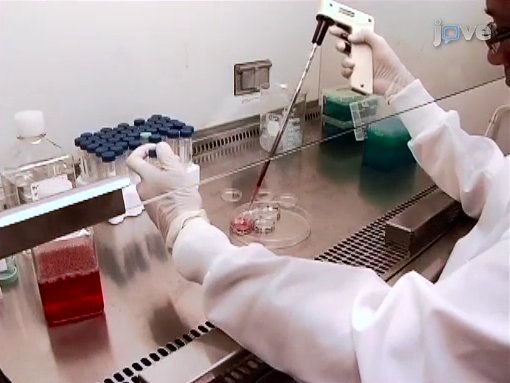
\includegraphics[width=0.45\textwidth]{chap1/figures/cells.png}
  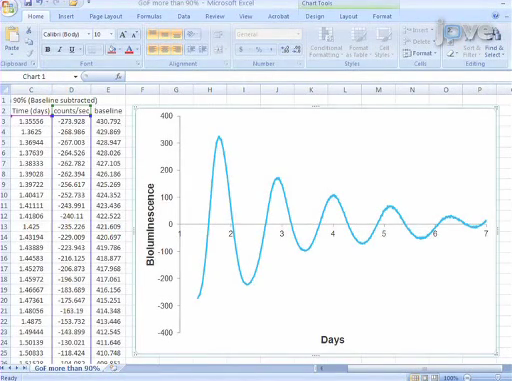
\includegraphics[width=0.45\textwidth]{chap1/figures/data.png}
  \titlecaption{Monitoring circadian parameters with bioluminescence reporter cell lines}{Cultured reporter cells allow parameters such as amplitude, period, and decay rate to be easily quantified. Image stills from \cite{Ramanathan2012}.}
  \label{fig:chidalumin}
\end{figure}

\section{Mathematical modeling}

Circadian rhythms, due to their dynamic nature, have long been the subject of mathematical inquiry \cite{Winfree2001}. In this section, I review some of the methods previously applied to understanding circadian rhythms.

\subsection{Introduction to modeling gene regulation}

Gene regulatory networks are typically modeled as dynamic systems, in which rates of production and degradation of each species is explicitly considered.
In \fref{fig:sysbiointro}, an example gene regulatory network is shown, in which a transcription factor activates the production of Gene 1. 
The genes mRNA is then translated to produce a protein product, which may or may not undergo posttranslational modifications or subcellular transport. 
The completed protein then modulates the production of a second mRNA for Gene 2.
In this example, the production and degradation rates of the mRNA and each protein state would be explicitly modeled.

\begin{figure}[tbp]
  \centering
  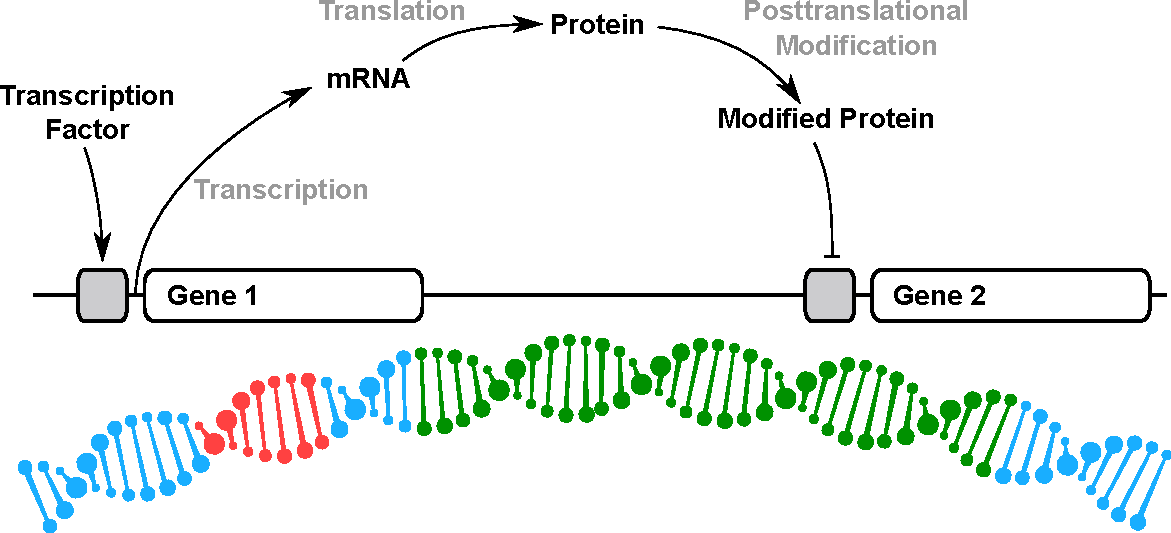
\includegraphics[width=\textwidth, clip=True, trim=0 100 0 0]{chap1/figures/sysbio_intro.pdf}
  \titlecaption{Gene regulatory networks can be modeled as dynamic systems}{Transcription, translation, degradation steps are treated as chemical reactions, in which the reaction rate depends only on the current concentration of other species and various kinetic parameters.}
  \label{fig:sysbiointro}
\end{figure}

If the values of the kinetic parameters (i.e., transcription rate) were known, the model could subsequently be simulated by casting the equations as either a system of ordinary differential equations (as in \fref{sec:odes}), or by using a chemical master equation (as in \fref{sec:stoch}). Resulting trajectories would resemble those shown in \fref{fig:extrajs}.

\begin{figure}[tbp]
  \centering
  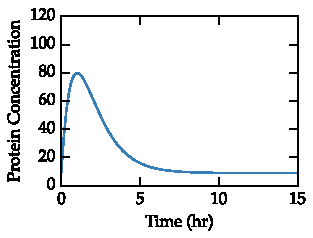
\includegraphics[width=0.475\textwidth]{chap1/figures/sysbio_trajs1.pdf}
  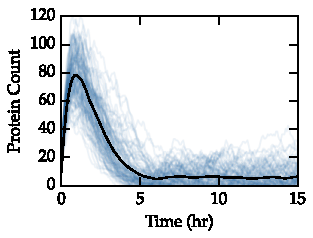
\includegraphics[width=0.475\textwidth]{chap1/figures/sysbio_trajs2.pdf}
  \titlecaption{Simulated time-dependent concentration trajectories}{(Left) Deterministic simulations of the dynamic system result in expected values for each state variable over time. (Right) Stochastic simulations account for the intrinsic noise present due to the low molecule counts of each reactant. From these simulations, more realistic noise estimates can be obtained at the expense of a greater computational complexity.}
  \label{fig:extrajs}
\end{figure}

\subsection{Ordinary differential equations}\label{sec:odes}

Ordinary differential equation (ODE) models take the general form
\begin{equation}
  \frac{dx}{dt} = f(x(t), p),
  \label{eq:odefn}
\end{equation}
in which $x(t)$ represents the concentrations of the state variables, such as mRNA and protein concentrations, $f$ contains information on the production, degradation, and reactivity of the states, and $p$ are the kinetic parameters which govern reaction kinetics.
Limit cycle models are ODE models in which the solution approaches a steady state oscillatory trajectory, satisfying the equation:
\begin{equation}
  \lim_{t \to \infty} \left[ x(t + T) - x(t) \right] = 0.
  \label{eq:limit5}
\end{equation}
The period is the smallest $T > 0$ for which \fref{eq:limit5} holds. 
An example periodic limit cycle is shown in \fref{fig:statespace}, which plots the deterministic solution to \fref{mod:novak}.

\begin{figure}[tbp]
  \centering
  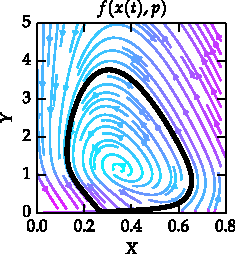
\includegraphics[width=0.45\textwidth]{chap1/figures/state_space.pdf}
  \titlecaption{State-space representation of a deterministic limit cycle}{A two-dimensional oscillator, \fref{mod:novak}, allows the system dynamics to be easily plotted. The steady state limit cycle, $x^\gamma(\theta)$, is shown in dark black. Points which lie off the limit cycle will eventually converge, following the vector field arrows. Colors represent the speed with which the solution will travel, with warmer colors indicating faster speeds.}
  \label{fig:statespace}
\end{figure}


The points on the stable limit cycle are denoted by $x^\gamma(\theta)$ with each point assigned to a value of a phase variable $\theta \in [0, 2\pi)$.
For convenience, time in \fref{eq:odefn} can be rescaled such that the period is $2\pi$:
\begin{equation}
  \tilde{t} = \frac{2\pi}{T}t; \quad \tilde{f} = \frac{T}{2\pi}\;f; \quad \frac{dx}{d\tilde{t}} = \tilde{f}(x(\tilde{t}), p).
  \label{eq:that}
\end{equation}
The phase variable $\theta$ is therefore defined on the limit cycle as $\theta = \tilde{t}\mod 2\pi$, with $\theta = 0$ assigned to a unique and identifiable point. An example mapping of the phase variable $\theta$ for \fref{mod:novak} is shown \fref{fig:phasedef}

\begin{figure}[tbp]
  \centering
  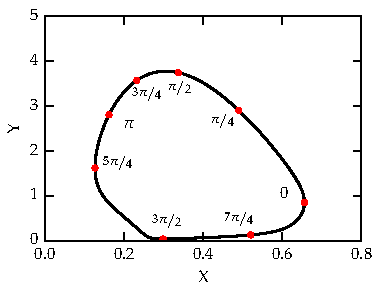
\includegraphics[width=0.5\textwidth]{chap1/figures/phase_def.pdf}
  \titlecaption{Definition of the phase variable}{A phase variable $\theta$ maps each point on the limit cycle, $x^\gamma(t)$, to a unique value of the phase. Because the definition of $\theta$ depends on time, the distance in state-space between each phase point is not equal.}
  \label{fig:phasedef}
\end{figure}


\subsection{ODE sensitivity analysis}

When analyzing ODE models, it is often important to know how the solution varies with respect to initial values or parameters. 
The sensitivity matrix is defined as
\begin{equation}
  S(t) = \frac{dx(t)}{dx(0)} = \lim_{\Delta x(0) \to 0}\frac{\Delta x(t)}{\Delta x(0)}.
  \label{eq:senslimit}
\end{equation}
While it is possible to obtain estimates of these derivatives through finite difference methods, more accurate and less computationally intensive representations can be obtained by integrating these sensitivities along with the original ODE system \cite{Dickinson1976}. 
The differential equation for the sensitivity system is shown in equation~\ref{eq:senslimit}. 
\begin{equation}
  \frac{d}{dt} S(t)  = \frac{df(x(t),p)}{dx}\; S(t)
  \label{eq:odesens}
\end{equation}
Since the jacobian matrix $\frac{\partial f}{\partial y}$ is the same as that of the original ODE system, efficient implementations of the following ODEs have been developed \cite{Feehery1997}.

\subsubsection{Period sensitivity}

An extension of sensitivity analysis for limit-cycle specific models raises additional complications. 
For instance, finding the derivative of the period with respect to parameter values requires a clever decomposition of the sensitivity matrices \cite{Kramer1984}. 
Period sensitivities, $\frac{\partial T}{\partial p}$, can be obtained directly from sensitivities integrated for one pass of the limit cycle (derived in \cite{Wilkins2009}) through a linear solve:
\begin{equation}
  \left[\begin{array}{cc}
      \mathbf{M} - \mathbf{I} & \dot{x}(T) \\
      \frac{\partial f_0}{\partial x}(x(0)) & 0
  \end{array}\right]
  \left[\begin{array}{c}
      \vdots \\ \frac{\partial T}{\partial p}
  \end{array}\right] =
  \left[\begin{array}{c}
      -\mathbf{S}(T) \\ -\frac{\partial {\bm f}}{\partial p}(x(0))
  \end{array}\right]
\end{equation}
in which $\mathbf{M}$ is the Monodromy matrix, $\mathbf{I}$ is the identity matrix, and the unknown vector contains the relevant period sensitivities.

Since parameter values often span several orders of magnitude, an often more useful measure is the relative period sensitivity, which is independent of the magnitude of the period or parameter value.
\begin{equation}
  \frac{\partial \ln T}{\partial \ln p} = \frac{p}{T}\frac{\partial T}{\partial p} = \frac{\partial T}{T} \left/ \frac{\partial p}{p} \right.
\end{equation}
Thus, a relative period sensitivity of 1 indicates that a 1\% increase in the parameter value will result in a 1\% increase in the period.

\subsubsection{Phase sensitivity}

Perturbations to state variables away from a limit cycle ultimately return, but with in a change of phase.
The definition of phase can be extended to points outside the limit cycle, $x_0 \not\in x^\gamma(\theta)$, by defining the phase of any point, $\Theta(x_0)$, as the initial phase of a point on the limit cycle to which $x_0$ will ultimately converge:
\begin{equation}
  \Theta(x_0) = \arg\min_\theta \lim_{t \to \infty} \lVert x(t)
  - x^\gamma(\theta + t)\rVert
  \label{eq:extendedphase2}
\end{equation}
A phase response curve (PRC), which maps the change in phase resulting from the same
perturbation applied at every phase, can therefore be found by calculating $
\Delta\theta \coloneqq \Theta(x^\gamma(\theta_0) + \Delta x(0)) - \theta_0$ for each
$\theta_0$. Infinitesimal PRCs, the derivative of the phase
change with respect to the perturbation, are defined for state and
parameter-impulse perturbations as \cite{Taylor2008a}:
\begin{align}
  \frac{d\theta}{dx} &\coloneqq \lim_{\Delta x(0) \to 0} \frac{\Delta\theta}{\Delta
  x(0)} \label{eq:sPRC}\\
  \frac{d}{d\hat{t}}\frac{d\theta}{dp} &\coloneqq \lim_{d,\; \Delta p \to 0}
  \frac{\Delta\theta}{d \; \Delta p}
  \label{eq:PRC}
\end{align}
Methods for efficiently calculating these quantities using ODE sensitivity
analysis have been developed \cite{Taylor2008a}, with the important result
that, in the limit as $d, \Delta p \to 0$, 
\begin{equation}
  \frac{d}{d\hat{t}}\frac{d\theta}{dp} = \frac{d\theta}{dx}\frac{d\hat{f}}{dp} 
  \label{eq:pPRCequiv}
\end{equation}

\subsection{Common kinetic assumptions}\label{sec:kinetic}

In constructing an ODE model of a genetic regulatory network, several common kinetic motifs are employed to capture various types of activation, repression, degradation, and complex formation.
In this section, I provide an overview of the kinetic assumptions used for model construction in subsequent chapters.

\subsubsection{Mass action law}

First developed approximately 150 years ago \cite{Voit2015}, the law of mass action is used for all types of chemical systems and forms the basis for subsequent kinetic constructions. 
In mass action kinetics, the reaction rate is proportional to the product of the activities (i.e. concentration) of each reactant.
For example, in the reversible reaction
\[
  A + B \xrightleftharpoons[k_{-1}]{k_{+1}} C,
\]
the reaction rates for the forward and reverse reactions ($r_{+1}$ and $r_{-1}$, respectively) would be
\begin{align*}
  r_{+1} &= k_{+1}[A][B]\\
  r_{-1} &= k_{-1}[C].
\end{align*}
As one molecule of $A$ and $B$ are consumed for each molecule of $C$ produced (and vice-versa for the reverse reaction), the ODE system describing this reaction would be:
\begin{align*}
  \frac{d[A]}{dt} &= k_{-1}[C] - k_{+1}[A][B]\\
  \frac{d[B]}{dt} &= k_{-1}[C] - k_{+1}[A][B]\\
  \frac{d[C]}{dt} &= k_{+1}[A][B] - k_{-1}[C],
\end{align*}
which reaches a fixed point (equilibrium) when $\nicefrac{d[\cdot]}{dt} = 0$, yielding the familiar expression for an equilibrium constant:
\[
  K_{eq} = \frac{k_{+1}}{k_{-1}} = \frac{[C]}{[A][B]}.
\]

\subsubsection{Michaelis-Menten Kinetics}\label{sec:mmenten}

The Michaelis-Menten rate law, first published in 1913 \cite{Johnson2011}, is a commonly used assumption to simplify the kinetics of an enzyme-mediated process.
The full system considered by the Michaelis-Menten model involves the reversible binding of an enzyme to a substrate, and the subsequent irreversible reaction of the enzyme-substrate complex, forming the product:
\begin{equation}
  E + S \xrightleftharpoons[k_r]{k_f} ES \xrightarrow{k_{cat}} E + P.
  \label{eq:mmreactions}
\end{equation}
The full ODE system for \fref{eq:mmreactions} is therefore
\begin{align}
  \frac{d[S]}{dt} &=  -k_f[E][S] \label{eq:S}\\
  \frac{d[E]}{dt} &= k_{cat}[ES] + k_r[ES] - k_f[E][S] \label{eq:E}\\
  \frac{d[ES]}{dt} &= k_f[E][S] - k_r[ES] - k_{cat}[ES] \label{eq:ES}\\
  \frac{d[P]}{dt} &= k_{cat}[ES]. \label{eq:P}
\end{align}
Since the concentration of enzyme-substrate complex, $[ES]$ is often difficult to measure experimentally, the above system of equations is typically not applied to real data.
Instead, a pseudo-steady state assumption (PSSA) is made, in which the equilibrium $E + S \xrightleftharpoons[k_r]{k_f} ES$ is assumed to equilibrate much faster than the product formation, $ES \xrightarrow{k_{cat}} E + P$.
This assumption results in $\nicefrac{d[ES]}{dt} \approx 0$, which can be used to simplify the above set of equations. 
We also assume a conservation of enzyme mass, $[E_T] = [E] + [ES]$. 
By solving the now-algebraic equations \ref{eq:E}-\ref{eq:ES} for $[E]$ and $[ES]$ and substituting the resulting expression into the remaining equations, we obtain:
\[
  [ES] = \frac{[E_T][S]}{\nicefrac{k_r}{k_f} + [S]}
\]
from which the production rate of the product is determined:
\begin{align*}
  \frac{d[P]}{dt} = \frac{V_{max}[S]}{K_M + [S]}, & & V_{max} = k_{cat}E_T, & \quad K_M = \frac{k_r}{k_f}.
\end{align*}
While the Michaelis-Menten model is widely used for enzyme-catalyzed reactions in biology, some articles have argued that the assumptions are likely not valid for protein-protein interactions, in which the substrate and enzyme are present in comparable concentrations \cite{Tzafriri2004}.

\subsubsection{Enzyme inhibition}
The Michaelis-Menten kinetic assumption can be extended to model the effects of enzyme inhibitors.
Different types of enzyme inhibition are possible, in which an inhibitor $I$ binds to the free enzyme $E$ and/or the enzyme-substrate complex.
In competitive inhibition, the inhibitor binds only to the free enzyme complex, blocking the binding of the substrate.
\begin{equation}
  E + I \xrightleftharpoons[k_{-i}]{k_{i}} EI
  \label{eq:compinh}
\end{equation}
Adding \fref{eq:compinh} to \fref{eq:mmreactions} and invoking the PSSA once more, we find the final rate for the conversion of substrate to product:
\begin{align}
  \frac{d[P]}{dt} = \frac{V_{max}[S]}{K_M\left(1 + \frac{[I]}{K_I}\right) + [S]}; & & K_I = \frac{k_{-i}}{k_i}.\label{eq:inheq}
\end{align}

\subsubsection{Hill-type kinetics}

In biochemical systems, cooperative binding between species is often required to initiate a reaction. 
The kinetics of such systems follow a sigmoidal profile, in which a critical amount of reactant species is required before significant product formation is seen, but which quickly saturates to a maximum value. 
The equation describing cooperative binding behavior was developed in 1910 \cite{Hill1910}. Assuming the conversion of reactant $S$ to product $P$, the rate of production of $P$ would follow
\begin{equation}
  \frac{d[P]}{dt} = \frac{V_{max} [S]^n}{K_A^n + [S]^n}
  \label{eq:hill}
\end{equation}
Depending on the degree of cooperativity $n$, the sigmoidal profile can vary between a standard Michaelis-Menten profile (no cooperativity) to an almost digital switch, as shown in \fref{fig:hillshapes}.
Hill-type kinetics can also include enzyme inhibition, in which the $K_A$ parameter would be scaled by inhibitor concentration in a manner similar to \fref{eq:inheq}.

\begin{figure}[tbp]
  \begin{center}
    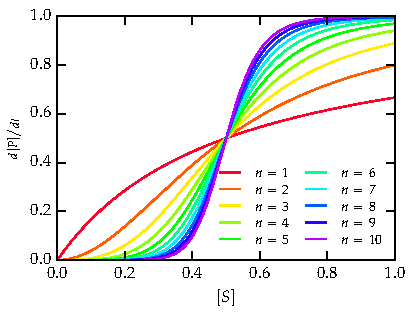
\includegraphics[width=0.6\textwidth]{chap1/figures/hilleq.pdf}
  \end{center}
  \titlecaption{Example profiles of the hill equation for various degrees of cooperativity}{The hill equation describes the kinetics of a cooperative reaction process, as shown in \fref{eq:hill}. Here $K_A = 0.5$, $V_{max} = 1$.}
  \label{fig:hillshapes}
\end{figure}


\subsection{Stochastic methods}\label{sec:stoch}

In modeling a system of chemical reactions using ODE methods, the assumption is made that the concentration of reacting species can take any continuous value. 
While this assumption is often appropriate for reactions in large, well-mixed vessels, it is often not the case in reactions that take place in the cell.
In mammalian cells, the median number of mRNA transcripts per cell is $17$, while the median number of protein copies is $50,000$ \cite{Schwanhausser2011}.
As a result, low concentrations of state variables are often best represented by discrete steps, in which the probabilistic nature of reaction events plays a large role in determining the system dynamics.

Stochastic systems are specified by a state vector of discrete populations $x = \{x_1, \ldots, x_N\}$ and reaction vector $R = \{R_1, \ldots, R_M\}$. 
For each of $M$ reactions, a stoichiometric vector $v_i$ describes the states which are produced and consumed by each reaction, and a reaction propensity function $a_i$ describes the likelihood of the reaction in for time step \cite{Gillespie1977}.
Together, these equations form the chemical master equation, a Markov (memoryless) process which can be efficiently simulated using a variety of algorithms \cite{Sanft2011}.


\subsection{Parameter estimation}

Models are typically used to validate that our assumed mechanisms are mathematically feasible, and to systematically explore consequences of our kinetic assumptions.
When these models differ from experimental results, we must re-analyze which of our assumptions might be incorrect and design new experiments to test these assumptions.
While biological insight is typically sufficient to construct candidate models $f(x, p)$ using standard assumptions outlined in \fref{sec:kinetic}, values for the kinetic parameters are typically derived by fitting experimental data.
In this section, I describe optimization techniques which have proven successful in finding descriptive parameter sets for models of circadian rhythms.

\subsubsection{Cost function}

The first step in finding a suitable parameter set is defining a cost function, $C(p)$, which ascribes a value to how well a particular parameter set fits the data.
By convention, the optimum parameter set is that which minimizes $C(p)$.
While for many biological systems a suitable cost function is the squared error of the model, a cost function can also include information on model derivatives, oscillatory period, and timing of various events (i.e., peak gene expression).
Cost functions of limit cycle models pose a particularly difficult optimization challenge, as a limit cycle does not always exist for any given parameter set.
Thus, the fitness landscape for most parameter space is very flat where limit cycle solutions do not exist, with isolated regions of  where limit cycle oscillations are possible.
Additionally, solving for the limit cycle solution given a parameter set is a nested optimization problem, resulting in long computation times.
For these reasons, stochastic global optimization procedures are often employed which efficiently search high dimensional parameter space without the need for derivative information of $C(p)$.
An overview of the computational approach typically employed for such systems is given in \fref{fig:comploop}.

\begin{figure}[tbp]
  \centering
  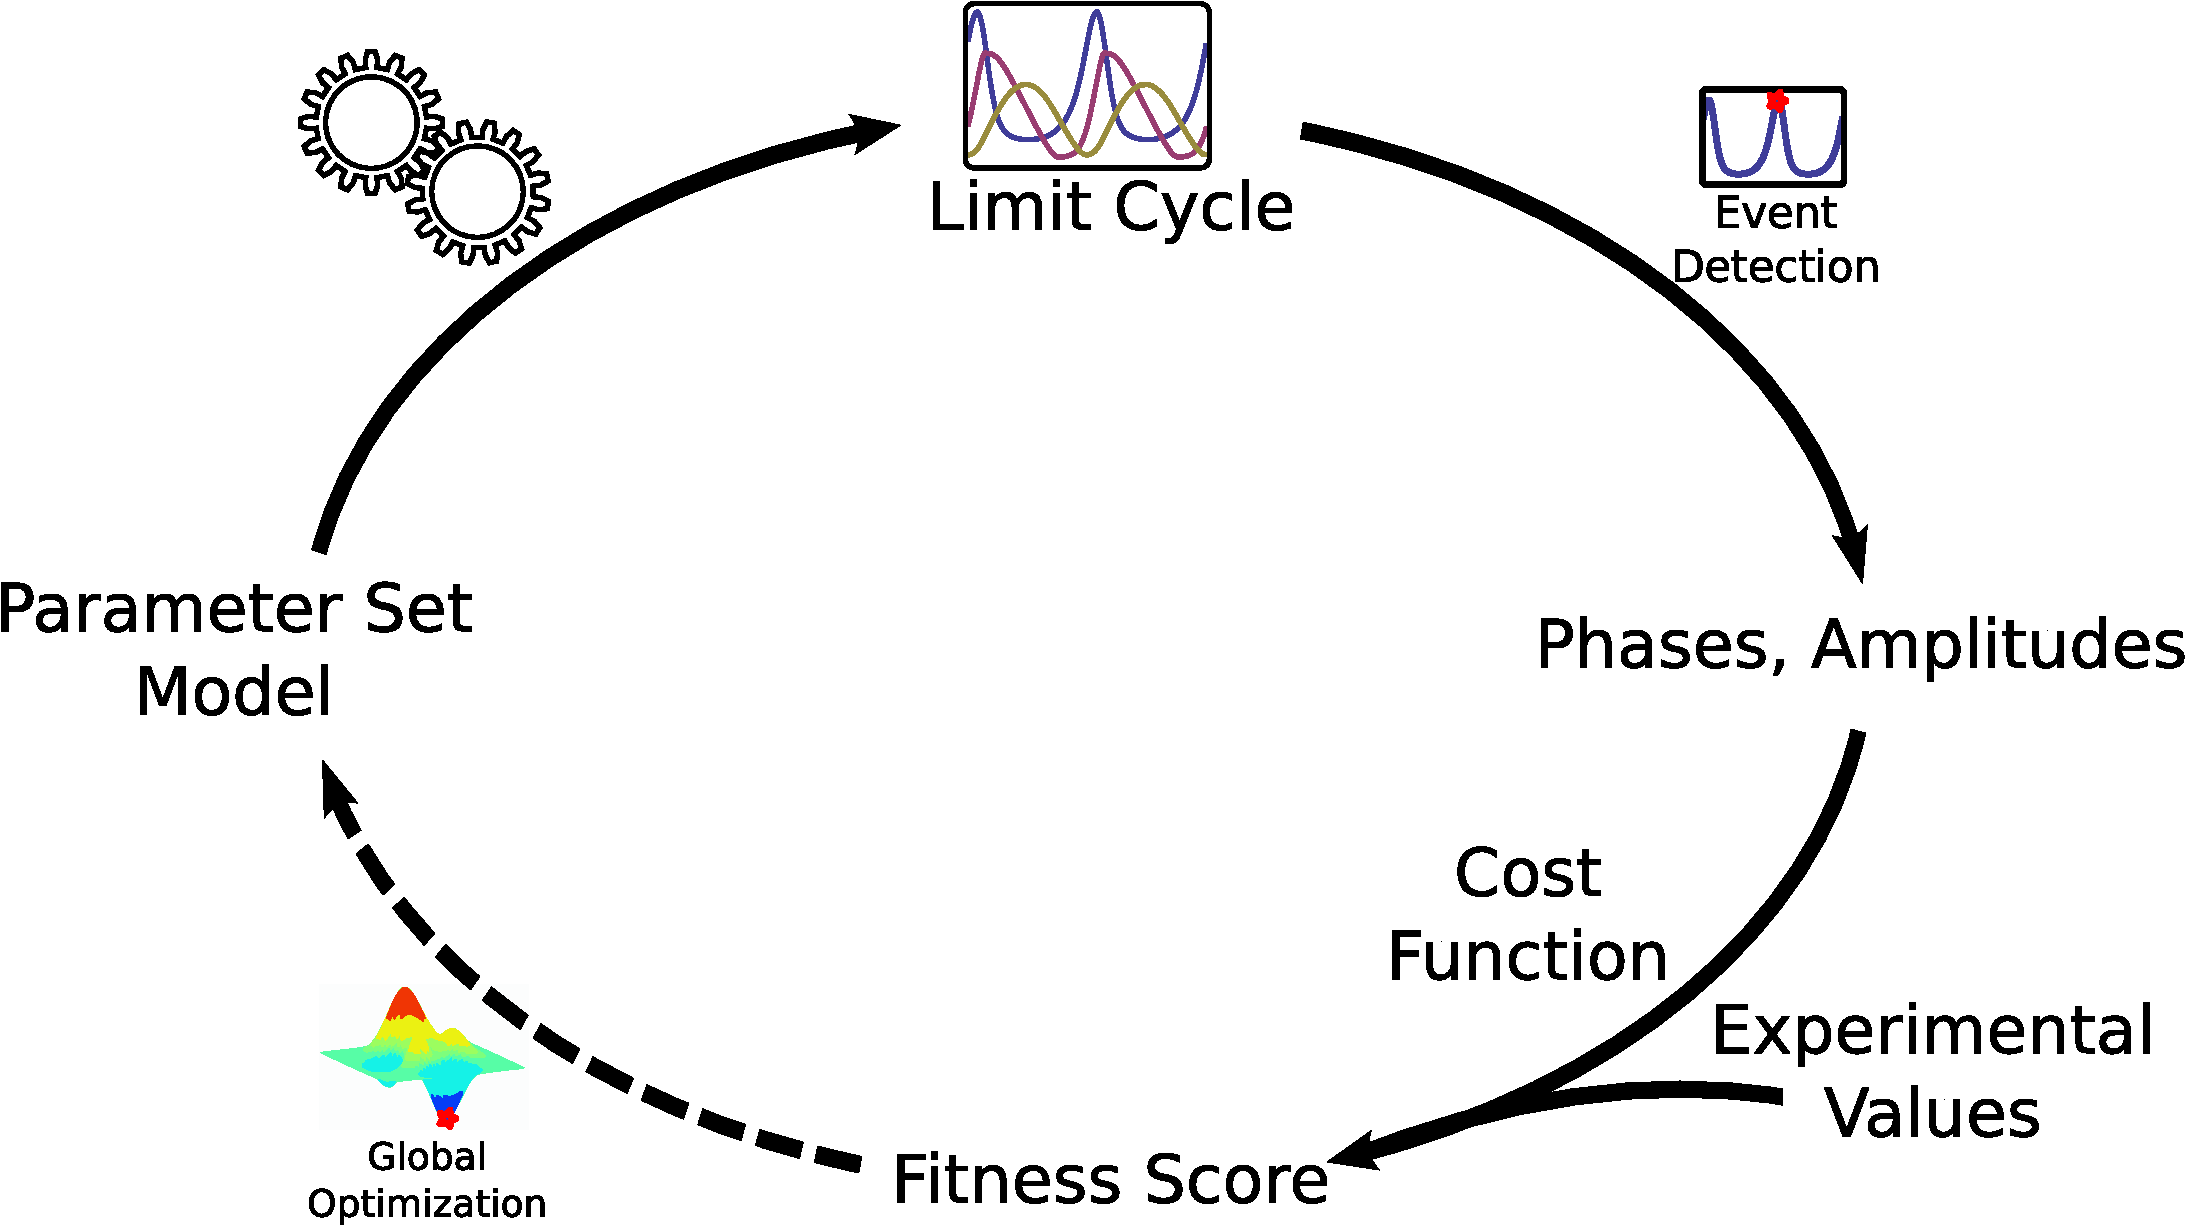
\includegraphics[width=0.65\textwidth]{chap1/figures/comp_loop.pdf}
  \titlecaption{An overview of the nested optimization of fitting limit cycle models}{Given a model and parameter set guess, a limit cycle is calculated via a single-shooting approach. A cost function then scores the timing of peak mRNA and protein species against known experimental values. Given the fitness score of many parameter guesses, a global optimization algorithm iteratively improves the parameter guess to minimize the cost function.}
  \label{fig:comploop}
\end{figure}

\subsubsection{Global optimization}
In this thesis, global optimization of model parameters is typically achieved via an evolutionary algorithm approach \cite{Whitley2001}. 
An evolutionary algorithm iteratively improves a parameter guess in an easily-parallelized fashion by mimicking natural evolution.
The steps involved are as follows, shown schematically in \fref{fig:gaoverview}.
\begin{enumerate}
  \item {\bfseries Initialization} An initial population of parameter guesses are generated from all parameter values, typically by a random number generation.
  \item {\bfseries Selection} The fitnesses (inverse of the cost) of the current population are evaluated, and a subsample of the original population is selected. A selection algorithm must randomly select from the current population, with some degree bias given towards individuals with the highest fitness.
  \item {\bfseries Crossover} Each member of the subsequent generation of solutions is generated by combining features from two (or more) of the selected individuals in the previous generation. For a problem consisting of many individual parameters, a common choice is to randomly select each parameter from one parent or the other.
  \item {\bfseries Mutation} The final step involves adding a small chance to change a parameter in the child parameter set. For continuous parameter values, this is often implemented as a small chance to add normally-distrusted error to one or more of the parameter values.
\end{enumerate}

\begin{figure}[tbp]
  \centering
  \begin{tabular}{cccc}
    \bf Initialization & \bf Selection & \bf Crossover & \bf Mutation \\
    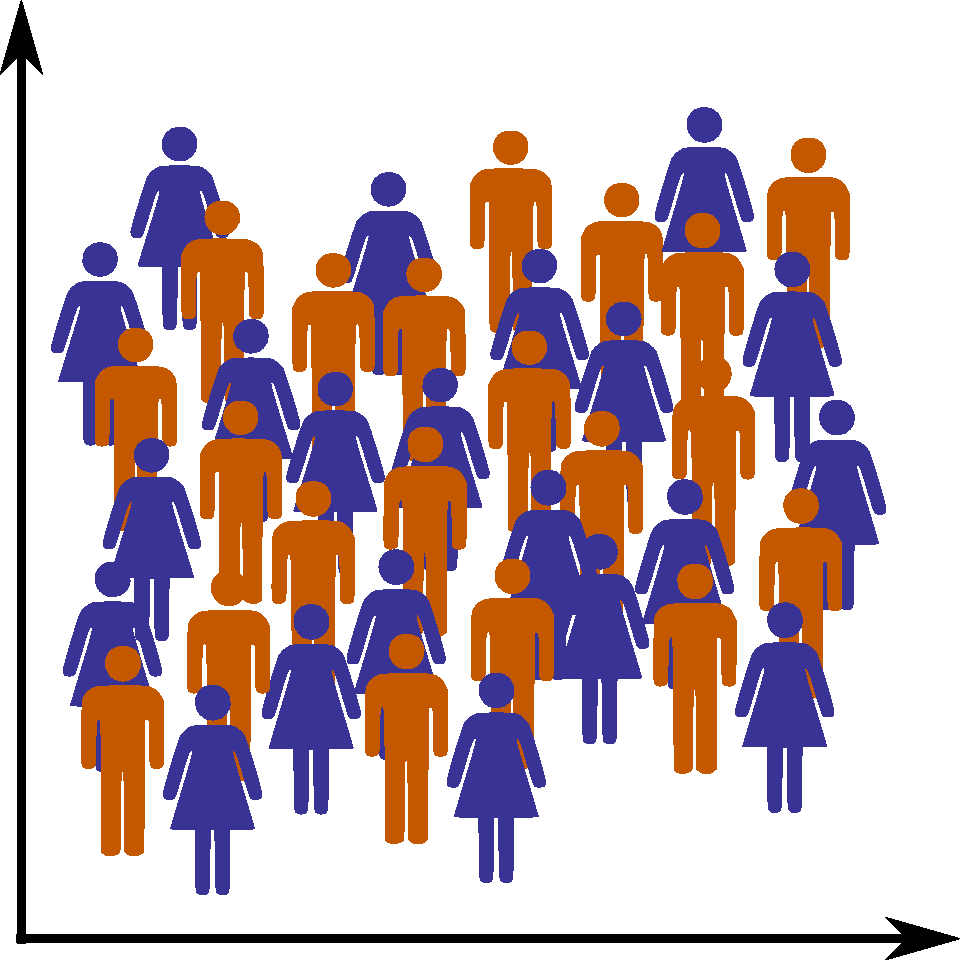
\includegraphics[width=0.2\textwidth]{chap1/figures/ga_initialization.pdf} &
    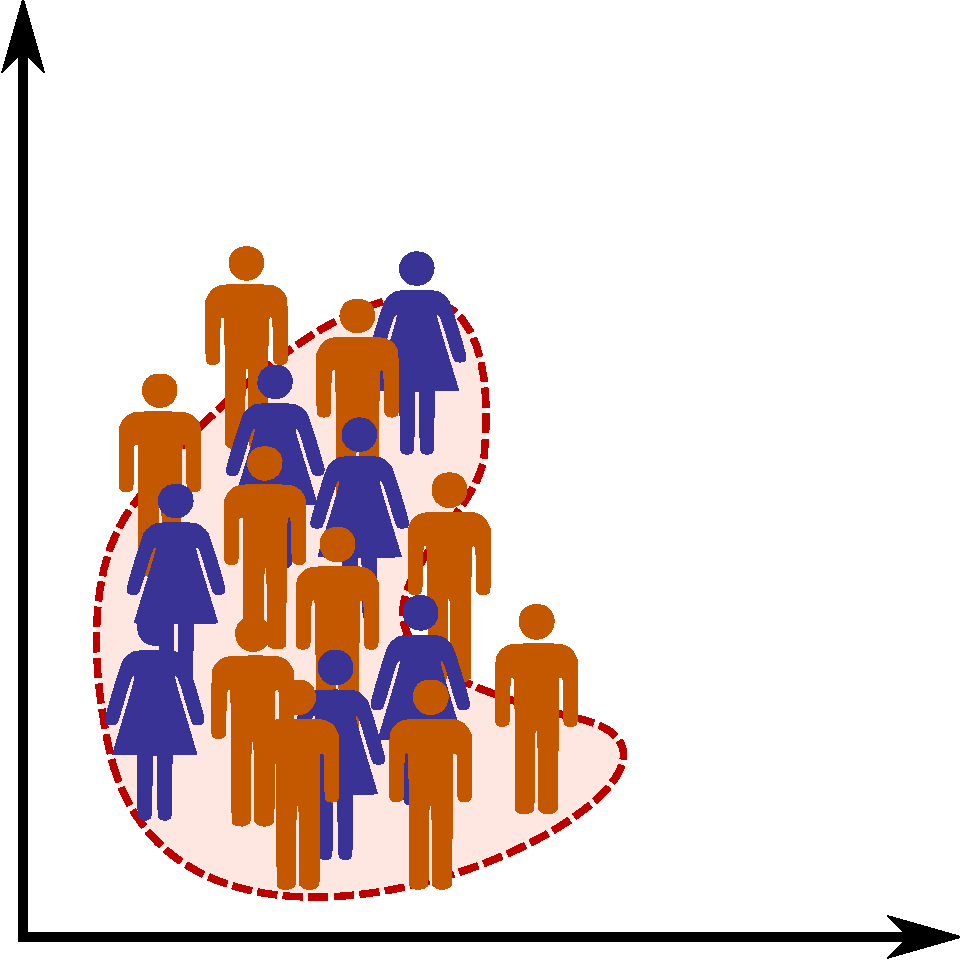
\includegraphics[width=0.2\textwidth]{chap1/figures/ga_selection.pdf} &
    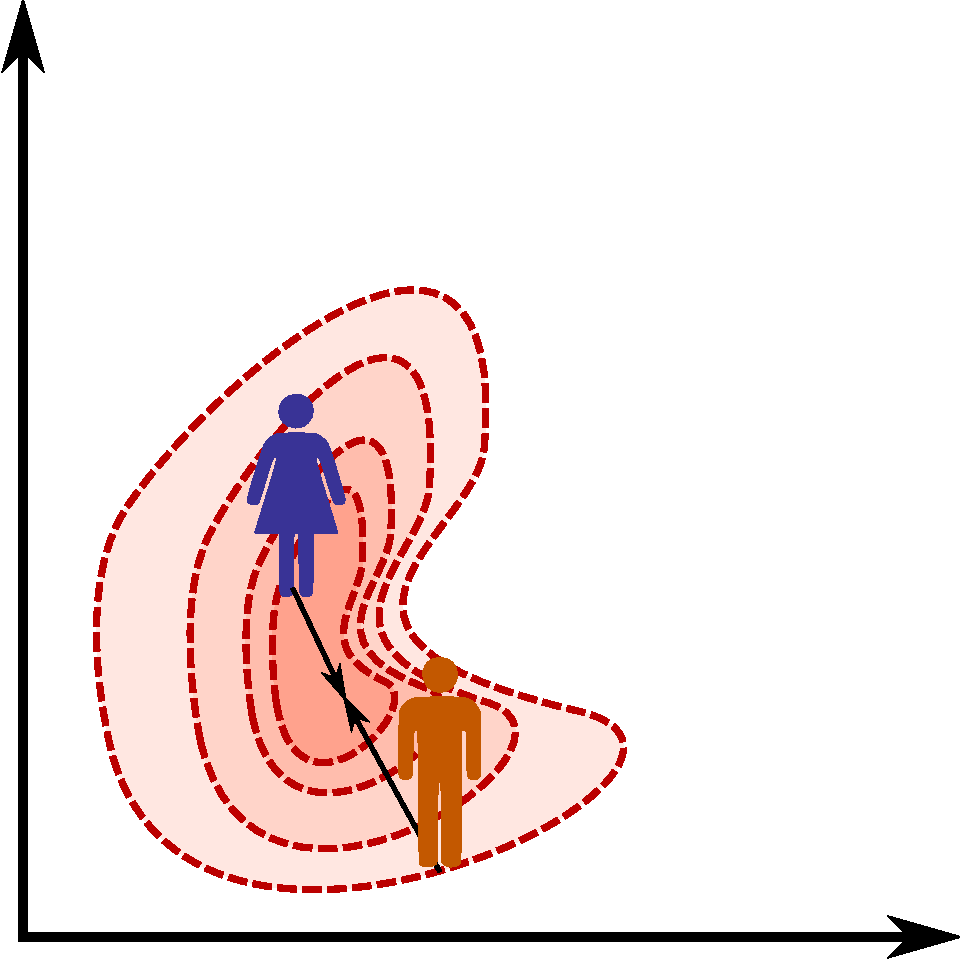
\includegraphics[width=0.2\textwidth]{chap1/figures/ga_crossover.pdf} &
    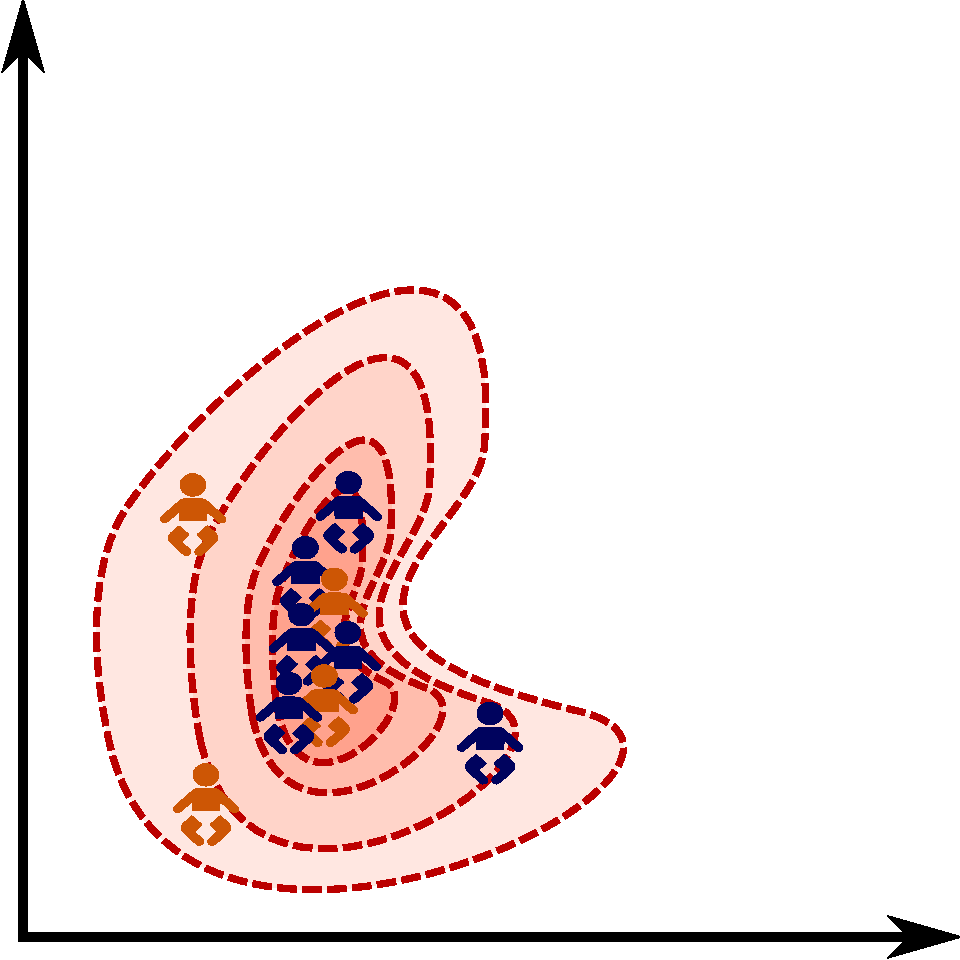
\includegraphics[width=0.2\textwidth]{chap1/figures/ga_mutation.pdf}\\
  \end{tabular}
  \titlecaption{An overview of global optimization via evolutionary strategy}{A schematic of a two-dimensional parameter space is shown. Solutions are initially distributed randomly across the parameter landscape, but solutions with a high fitness are preferentially kept. By combining and slightly altering parameter values from existing solutions, each generation iteratively approaches the highest fitness.}
  \label{fig:gaoverview}
\end{figure}

\subsection{Previous models of circadian rhythms}

Since mathematical methods have been used to study circadian rhythms for some time, many existing models of circadian gene regulation exist.
Early examples include Goodwin's 1965 model of enzymatic oscillations, demonstrating that nonlinear oscillations could capture many of the features of biological rhythms \cite{Goodwin1965}. 
Later models sought to describe specific proteins in the circadian cycle. 
Goldbeter's 1995 model described one gene in the circadian clock of {\it Drosophila}, and demonstrated that a negative feedback loop with sufficient nonlinearity and time delay was required for circadian oscillations \cite{Goldbeter1995}.

Subsequent models have attempted to generate a more complete representation of the circadian network. 
Leloup and Goldbeter's 2003 model of the mammalian circadian clock considers both the positive and negative regulatory loops \cite{Leloup2003}, demonstrating the anti-phase oscillations of the positive and negative elements. 
Forger and Peskin's 73-state model, and its analogous stochastic version, provides an example of the complexity of the known post-translational regulation of core clock components \cite{Forger2003,Forger2005}.

More recently, models have focused on explaining new theories on how circadian rhythms are organized, rather than attempting to providing a complete {\itshape in silico} representation of current knowledge.
A model by To {\itshape et al.,} 2007 coupled together cells modeled by Leloup \& Goldbeter's 2003 model to demonstrate how heterogeneous populations of oscillators could synchronize in an SCN environment using the neurotransmitter vasoactive intestinal polypeptide (VIP) \cite{To2007}.
Following the differentiation between the properties of single-cell oscillators and populations, Mirsky {\itshape et al.,}, 2009 developed a model to show how single-cell knockout phenotypes could be differentiated from those at the population-level \cite{Mirsky2009}.
Rel{\'o}gio {\itshape et al.,} 2011 demonstrated that positive feedback through ROR/REV-ERB had a stabilizing effect on the clock \cite{Relogio2011}, while a model from Kim \& Forger, 2012 demonstrated the importance of stoichiometry between positive and negative components \cite{Kim2012}.

Despite the wide availability of mathematical models for circadian rhythms, demonstrating that new theories are mathematically rigorous often requires the creation of a new model. In the following chapter, I describe the process of model creation in more detail following new experimental insight into core clock dynamics.

